\chapter{Polynomials}\label{chapter:polynomials}

\section{Polynomials with Abstract Coefficients}

\begin{definition}
  An \emph{polynomial} in one variable $x$ is an expression of the form
  \begin{equation*}
    f(x) = a_nx^n+ a_{n-1}x^{n-1} +\cdots + a_0,
  \end{equation*}
  in which we require that the \emph{leading coefficient} $a_n$ is nonzero, unless $n=0$. A polynomial $f(x)$ as above with leading coefficient $a_n$ is said to be of \emph{degree} $n$. The numbers $a_k$ are called the \emph{coefficients} of $f(x)$. The \emph{zero polynomial} is the constant polynomial $f(x)=0$.
\end{definition}

The coefficients of a polynomial may be taken from any number system. When we wish to specify that the coefficients are integers, rational, or real numbers, we speak of \emph{polynomials with integer coefficients}, \emph{polynomials with rational coefficients}, or \emph{polynomials with real coefficients}. Other number systems from which we will occasionally take coefficients include the rings $\mathbb{Z}/n$ of modular arithmetic. Since there is such a large variety of number systems which will eventually play a role one way or another in number theory, it will be useful to us to develop methods general enough so as to cover all these cases at once.

\begin{definition}
  A \emph{commutative ring} is a set $R$ equipped with constants $0$ and $1$ and operations $+$ for addition, $-$ for subtraction, and $\cdot$ for multiplication, satisfying the following laws of arithmetic:
  \begin{align*}
    (x+y)+z & = x + (y+ z), & (xy)z & = x(yz), \\
    x + y & = y + x, & xy & = yx, \\
    0+x & = x, & 1x & = x, \\
    x+(-x) & = 0, & x(y+z) & = xy+xz.
  \end{align*}
  The adjective \emph{commutative} refers to the law asserting that $xy=yx$. A commutative ring with $0\neq 1$ is said to be a \emph{integral domain} if it satisfies the following condition:
  \begin{equation*}
    xy=0 \Rightarrow x=0\lor y=0.
  \end{equation*}
  A commutative ring with $0\neq 1$ is said to be a \emph{field} if it comes equipped with a further operation $({-})^{-1}$ defined on all nonzero elements, such that
  \begin{equation*}
    xx^{-1}=1.
  \end{equation*}
\end{definition}

Examples of commutative rings include most number systems we have encountered so far: $\mathbb{Z}$, $\mathbb{Q}$, and $\mathbb{Z}/n$ for any $n$. The Gaussian integers $\mathbb{Z}[i]$ are another important example of a ring. There is one important omission: The set of natural numbers with the usual operations of addition and multiplication is not a ring because it lacks subtraction.

The sharp reader may have observed that some laws of arithmetic, such as $0x=0$, are not stated in the definition of a (commutative) ring. Indeed, this law can be proven:
\begin{equation*}
  0x=0x+0=0x+(0x-0x)=(0x+0x)-0x=(0+0)x-0x=0x-0x=0.
\end{equation*}
Most rings satisfy the condition that $0\neq 1$. Indeed, if $0=1$ in a ring $R$, then any element equals $0$ because
\begin{equation*}
  x=1x=0x=0.
\end{equation*}
Thus, only the ring $\mathbb{Z}/1$ satisfies $0=1$. This ring is called the \emph{trivial ring} for understandable reasons.

The condition of being an integral domain is quite innocent-looking: It guarantees that the product of any two nonzero numbers is nonzero. This condition is true in familiar number systems such as $\mathbb{Z}$, $\mathbb{Z}[i]$, $\mathbb{Q}$, and $\mathbb{R}$, which are therefore integral domains. However, the ring $\mathbb{Z}/n$ is only an integral domain when $n$ is prime. For composite $n$, we can find examples of nonzero numbers that multiply to $0$. For instance, we have $2\cdot 2\equiv 0\pmod{4}$ in $\mathbb{Z}/4$, and we have $2\cdot 3\equiv 0\pmod{6}$ in $\mathbb{Z}/6$. Having such examples shows that the condition of being an integral domain is not provable from the laws of arithmetic stated in the definition of a ring.

Of the examples we have seen so far, only $\mathbb{Q}$ and $\mathbb{Z}/p$ are fields. Other familiar fields include the field $\mathbb{R}$ of real numbers and the field $\mathbb{C}$ of complex numbers. We note that any field is an integral domain: If $xy=0$ and $x\neq 0$, then $x$ has a multiplicative inverse. This allows us to calculate as follows and find that
\begin{equation*}
  y=1y=(x^{-1}x)y=x^{-1}(xy)=x^{-1}0=0.
\end{equation*}

The previous definitions of rings, integral domains, and fields are extremely general. There are many examples of rings that have little to do with numbers, except that they satisfy the laws of arithmetic. We stress here that our goal is not to develop the general theory of rings, where we would have to be concerned with the vast scope of the subject. Instead, our goal is simply to avoid having to reprove essentially the same theorems about polynomials separately for polynomials with integer coefficients, rational coefficients, real coefficients, and so on. By stating them in terms of polynomials with coefficients in a ring or integral domain, we cover all those cases at once.

\begin{remark}
  There is another subtle, yet important aspect of polynomials which needs to be emphasized: The distinction between polynomials and the functions they describe. This distinction comes to light when considering equality of polynomials. Two polynomials
  \begin{equation*}
    a_nx^n+ a_{n-1}x^{n-1} +\cdots + a_0\qquad\text{and}\qquad b_nx^n+ b_{n-1}x^{n-1} +\cdots + b_0
  \end{equation*}
  are said to be equal if their coefficients are equal, meaning that $a_i=b_i$ for all $0\leq i\leq n$, while functions are considered equal if their values are equal. This is an important distinction, because for some number systems such as the integers modulo $n$, polynomials aren't necessarily equal as polynomials when they are equal as functions. For instance, by \crefnamed{theorem:fermats-little-theorem} we have that
  \begin{equation*}
    x^p \equiv x\pmod{p},
  \end{equation*}
  while the polynomials $x^p$ and $x$ clearly can be distinguished by their coefficients. Nevertheless, we will show in \cref{corollary:extensionality-integer-polynomials} that two polynomials with integer coefficients have equal coefficients if and only if they define equal functions.
\end{remark}

\begin{definition}
  Consider a ring $R$. A function $f:R\to R$ is said to be \emph{polynomial in $R$} if there exists a polynomial with coefficients in $R$ such as the above, such that
  \begin{equation*}
    f(x)=a_nx^n+ a_{n-1}x^{n-1} +\cdots + a_0
  \end{equation*}
  for all $x\in R$.
\end{definition}

\begin{remark}
  Polynomials can be added, subtracted, and multiplied in the same way as integers. To add two polynomials, we add their corresponding coefficients, taking missing coefficients as zero when necessary. Polynomials are multiplied by the formula
  \begin{align*}
    \Biggl(\sum_{i=0}^n a_ix^i\Biggr)\Biggl(\sum_{j=0\vphantom{i=0}}^mb_jx^j\Biggr)
    & = \sum_{i=0}^n\sum_{j=0}^ma_ib_jx^{i+j} \\
    & = \sum_{k=0}^{n+m}\sum_{i=0}^n a_i b_{k-i}x^{k}.    
  \end{align*}
  These operations of addition, subtraction, and multiplication of polynomials satisfy the laws of arithmetic. More precisely, the polynomials with coefficients in a commutative ring form itself a commutative ring.
\end{remark}

\section{The Factor Theorem}

\begin{definition}
  Consider a polynomial $f(x)$ with coefficients in a ring $R$. A \emph{root} of $f(x)$ is an element $r\in R$ such that
  \begin{equation*}
    f(r)=0.
  \end{equation*}
  Sometimes we will write $N(f)$ for the set of roots of $f$.
\end{definition}

In the following theorem we will prove that if $r$ is a root of the polynomial $f(x)$, then we can factor $f(x)$ as $(x-r)g(x)$. This theorem applies for polynomials in any commutative ring.

\begin{theorem}[Factor Theorem]\label{theorem:factor-theorem}
  Consider a ring $R$, and a nonzero polynomial $f(x)$ of degree $n$ with coefficients in $R$.
  An element $r\in R$ is a root of $f(x)$ if and only if there is a polynomial $g(x)$ of degree $n-1$ with coefficients in $R$ such that $f(x)=(x-r)g(x)$.
\end{theorem}

\begin{proof}
  We will prove the claim by induction on $n$. In the base case $f(x)$ is a nonzero constant polynomial, so it has no roots and there is nothing to prove.

  For the inductive step, it is clear that if there is a polynomial $g(x)$ such that $f(x)=(x-r)g(x)$, then $r$ is a root of the polynomial $f(x)$. For the converse, suppose that $r$ is a root of $f(x)$. Then
  \begin{equation*}
    f(x) = f(x)-f(r) = a_n(x^n-r^n)+\cdots + a_1(x-r).
  \end{equation*}
  By the formula for the difference of $k$th powers, which was stated in \cref{exercise:difference-of-powers} and which holds in any ring, we can factor $x^k-r^k$ as
  \begin{equation*}
    x^k-r^k=(x-r)q_k(x),\qquad\text{where}\qquad q_k(x)=\sum_{i=0}^{k-1}x^ir^{k-1-i}
  \end{equation*}
  is a polynomial of degree $k-1$. Now define $g(x) := \sum_{k=1}^{n}a_k q_k(x)$. Then we compute
  \begin{equation*}
    (x-r)g(x)=\sum_{k=1}^{n}a_k (x-r)q_k(x)=\sum_{k=1}^{n}a_k (x^k-r^k)=f(x)-f(r)=f(x).\qedhere
  \end{equation*}
\end{proof}

\crefnamed{theorem:factor-theorem} has some important corollaries. One of them states that in an integral domain, where the product of any two nonzero numbers is guaranteed to be nonzero, any polynomial of degree $n$ has at most $n$ roots.

\begin{corollary}\label{corollary:number-of-roots-polynomial}
  Consider an integral domain $R$. A polynomial of degree $n$ with coefficients in $R$ has at most $n$ roots.
\end{corollary}

\begin{proof}
  The proof is by induction on the degree $n$. If $f(x)$ is a constant polynomial of degree $0$ and its leading coefficient is nonzero, then $f(x)$ is always nonzero and so $f(x)$ has no roots.

  For the inductive step, assume that all polynomials of degree $n$ have at most $n$ roots, and consider a polynomial $f(x)$ of degree $n+1$. Then either $f(x)$ has no roots, in which case we are done immediately, or $f(x)$ has a root $r$, in which case $f(x)$ factors as
  \begin{equation*}
    f(x)=(x-r)g(x)
  \end{equation*}
  by \crefnamed{theorem:factor-theorem}, where $g(x)$ is a polynomial of degree $n$. Since we assumed that $R$ is an integral domain, it follows that for any element $x\in R$, the identity $(x-r)g(x)=0$ holds in $R$ if and only if one of the identities $x-r=0$ or $g(x)=0$ holds in $R$. Thus we see that $x$ is a root of the polynomial $f(x)$ if and only if $x=r$ or $x$ is a root of the polynomial $g(x)$. We conclude that the polynomial $f(x)$ has at most $n+1$ roots.
\end{proof}

The Factor Theorem also raises an immediate question of uniqueness. If $f(x)$ and $g(x)$ are two polynomials, is there always at most one way in which we can write
\begin{equation*}
  f(x)=g(x)h(x)?
\end{equation*}

\begin{proposition}[Cancellation Law for Polynomials]\label{proposition:cancellation-law-polynomials}
  Let $f(x)$ be a nonzero polynomial with coefficients in an integral domain. Consider two polynomials $h(x)$ and $k(x)$ satisfying the identity of polynomials
  \begin{equation*}
    f(x)h(x)=f(x)k(x).
  \end{equation*}
  Then $h(x)=k(x)$. 
\end{proposition}

\begin{proof}
  By the assumption that $f(x)h(x)=f(x)k(x)$, it follows that
  \begin{equation*}
    f(x)(h(x)-k(x))=0.
  \end{equation*}
  Write $g(x):=h(x)-k(x)$. Note that all the coefficients of the polynomial $f(x)g(x)$ are $0$. However $f(x)$ is a nonzero polynomial, so it has a leading coefficient $a_n$. Now, suppose for a contradiction that $g(x)$ is nonzero, with leading coefficient $b_m$. Their product $f(x)g(x)$ has leading coefficient $a_nb_m$, which is nonzero since it is a product of nonzero elements of an integral domain. Hence $f(x)g(x)$ is nonzero, which is a contradiction.
\end{proof}

\section{Polynomial Congruences of Prime Moduli}

Even though a polynomial
\begin{equation*}
  f(x) = a_nx^n+ a_{n-1}x^{n-1} +\cdots + a_0
\end{equation*}
has at most $n$ roots in the integers, the same is not true in modular arithmetic. A fairly easy example, the quadratic congruence
\begin{equation*}
  x^2 \equiv 1\pmod{8}
\end{equation*}
has four solutions, the numbers $1$, $3$, $5$, and $7$. On the other hand, we will prove in this section that the number of solutions of a polynomial congruence modulo a prime is, just as in the integer case, at most the degree of the polynomial.

\begin{theorem}[Factor Theorem in Modular Arithmetic]\label{theorem:factor-theorem-modular-arithmetic}
  An integer $r$ is a solution to the polynomial congruence
  \begin{equation*}
    f(x) \equiv 0\pmod{n},
  \end{equation*}
  if and only if
  \begin{equation*}
    f(x) \equiv (x-r)g(x) \pmod{n}
  \end{equation*}
  for some polynomial $g(x)$.
\end{theorem}

\begin{proof}
  The proof is very similar to the proof of \cref{theorem:factor-theorem}. First, we note that the converse direction is trivial, so we focus on the forward direction. Suppose that
  \begin{equation*}
    f(r) \equiv 0 \pmod{n}
  \end{equation*}
  and consider the polynomial $f(x)-f(r)$. Then we have
  \begin{equation*}
    f(x)\equiv f(x)-f(r) \pmod{n},
  \end{equation*}
  and the factorization of $f(x)-f(r)$ as $(x-r)g(x)$ follows in the same way as for \cref{theorem:factor-theorem}.
\end{proof}

\begin{theorem}[Lagrange's Theorem]\label{theorem:lagranges-theorem}
  Consider a polynomial
  \begin{equation*}
    f(x) = a_nx^n+ a_{n-1}x^{n-1} +\cdots + a_0,
  \end{equation*}
  and a prime $p$ such that $p\nmid a_n$. Then the polynomial congruence
  \begin{equation*}
    f(x)\equiv 0 \pmod{p}
  \end{equation*}
  has at most $n$ solutions.
\end{theorem}

\begin{proof}
  We prove the claim by induction on the degree $n$ of the polynomial $f$. If $f$ has degree zero, then $f(x)=a_0$, and since the leading term of $f$ is assumed to be not divisible by $p$, it follows that $a_0\nequiv 0\pmod{p}$. Thus, the polynomial $f$ has no solutions modulo $p$.

  Now suppose that any polynomial congruence modulo $p$ of degree $n$ has at most $n$ solutions, and consider a polynomial congruence $f(x)\equiv 0\pmod{p}$ of degree $n+1$. If this congruence has no roots, then the number of solutions is certainly below $n+1$.

  On the other hand, if $f(r)\equiv 0\pmod{p}$ is a solution, then by \crefnamed{theorem:factor-theorem-modular-arithmetic} we can find a polynomial $g(x)$ of degree $n$ such that
  \begin{equation*}
    f(x)\equiv (x-r)g(x) \pmod{p}.
  \end{equation*}
  It follows that the polynomial congruences $f(x)\equiv 0\pmod{p}$ and
  \begin{equation*}
    (x-r)g(x)\equiv 0 \pmod{p}
  \end{equation*}
  have the same sets of solutions. Since $p$ is prime, we have by \cref{proposition:euclid-divisibility-primes} that $ab\equiv 0\pmod{p}$ if and only if $a\equiv 0\pmod{p}$ or $b\equiv 0\pmod{p}$. Any solution $x$ of the congruence $(x-r)g(x)\equiv 0\pmod{p}$ must therefore satisfy $x-r\equiv 0\pmod{p}$ or $g(x)\equiv 0\pmod{p}$. There are at most $d$ solutions of the polynomial congruence $g(x)\equiv 0\pmod{p}$, so we conclude that there are at most $d+1$ solutions to the polynomial congruence $f(x)\equiv 0\pmod{p}$.
\end{proof}

The previous theorem is due to Joseph-Louis Lagrange, published in 1770 in \emph{Réflexions sur la résolution algébrique des équations} \cite{lagrange1770}. Lagrange demonstrated that the roots of polynomials can be studied by their permutations. His ideas would eventually lead to the emergence of group theory (the study of symmetry), and Galois theory.

While \crefnamed{theorem:lagranges-theorem} establishes an upper bound for the number of incongruent solutions of a polynomial congruence modulo a prime, we can use \crefnamed{theorem:fermats-little-theorem} to find examples of polynomial congruences that have the maximum allowable number of solutions.

\begin{theorem}\label{theorem:maximal-number-of-roots-pow-minus-id}
  Consider a prime $p$ and a positive integer $n$ such that $n\mid p-1$. Then the polynomial congruence
  \begin{equation*}
    x^n\equiv 1\pmod{p}
  \end{equation*}
  has exactly $n$ incongruent solutions.
\end{theorem}

\begin{proof}
  Note that the polynomial congruence $x^{p-1}-1\equiv 0\pmod{p}$ has exactly $p-1$ solutions. By the formula for the difference of powers, we have
  \begin{equation*}
    (x^{p-1}-1)\equiv (x^n-1)q(x) \pmod{p}
  \end{equation*}
  for some polynomial $q$ of degree $p-1-n$. Now we observe that the polynomial congruences
  \begin{equation*}
    x^n-1\equiv 0\pmod{p}\qquad\text{and}\qquad q(x)\equiv 0\pmod{p}
  \end{equation*}
  have at most $n$ and $p-1-n$ solutions, respectively. Since their product has $p-1$ solutions, it follows that the polynomial congruence $x^n-1\equiv 0\pmod{p}$ must have exactly $n$ solutions.
\end{proof}

\crefnamed{theorem:lagranges-theorem} can also be used to give another proof of \cref{theorem:quadratic-character-neg-1}, which states that for an odd prime $p$, the quadratic congruence $x^2\equiv -1\pmod{p}$ has a solution if and only if $p\equiv 1\pmod{4}$.

\begin{proof}[Proof of \cref{theorem:quadratic-character-neg-1}]
  We prove that if $p\equiv 1\pmod{4}$, then there is a square root of $-1$ modulo $p$. Consider a prime $p$ of the form $4k+1$. Then \crefnamed{theorem:fermats-little-theorem} implies that
  \begin{equation*}
    (x^{2k}+1)(x^{2k}-1)=x^{4k}-1\equiv 0\pmod{p}.
  \end{equation*}
  Since $p$ is prime, this implies that $x^{2k}+1\equiv 0\pmod{p}$ or $x^{2k}-1\equiv 0\pmod{p}$ for every integer $x$. However, the polynomial congruence
  \begin{equation*}
    x^{2k}-1\equiv 0\pmod{p}
  \end{equation*}
  has at most $2k$ solutions modulo $p$, which is strictly fewer than $p$. Thus, there must exist an integer $x$ such that
  \begin{equation*}
    x^{2k}+1\equiv 0\pmod{p}.
  \end{equation*}
  Given such an integer $x$, we see that $y:=x^k$ is a square root of $-1$ modulo $p$.
\end{proof}

\section{Lagrange's Interpolation Theorem}

Lagrange's Interpolation Theorem establishes that for any set of data points, as illustrated in \cref{figure:lagrange-interpolation}, there is always a way of defining a polynomial that exactly matches the data. Moreover, it gives the unique way of defining such a polynomial in the lowest degree. Interpolation theorems such as Lagrange's or Newton's addressed a practical need for geometers of the $17th$ and $18th$ centuries: It allowed them to estimate intermediate values of a function from a finite amount of data such as tables of planetary positions or values of trigonometric functions.

Lagrange's Interpolation Theorem has the important consequence that any polynomial of degree $n$ is uniquely determined by any $n+1$ of its values. We will also use Lagrange's Interpolation Theorem in the next section to derive a divisibility property of polynomials due to Kurt Hensel.

\begin{figure}[t]
  \centering
  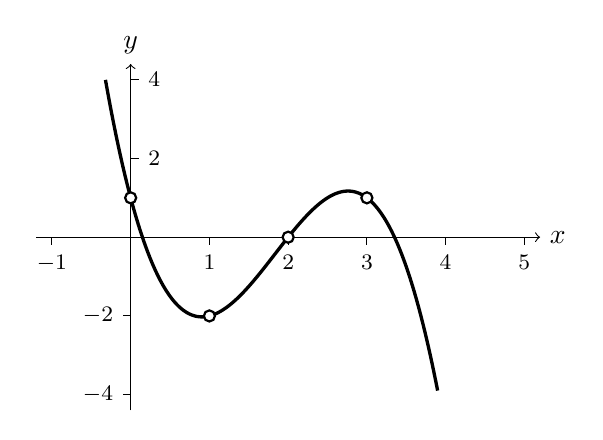
\begin{tikzpicture}
    [x=1cm,y=.5cm]
    \draw[->] (-1.2,0) -- (5.2,0) node[right] {$x$};
    \draw[->] (0,-4.4) -- (0,4.4) node[above] {$y$};

    \foreach \x in {-1, 1,2,3,4,5} {
      \draw (\x,0) -- (\x,-.2)
      node[below,font=\footnotesize] {$\x$};
    }

    \foreach \y in {-4,-2} {\draw (0,\y) -- (-.1,\y) node[left,font=\footnotesize] {$\y$};}

    \foreach \y in {2,4} {\draw (0,\y) -- (.1,\y) node[right,font=\footnotesize] {$\y$};}
          
    
    % Plot the interpolating polynomial
    \draw[very thick, domain=-0.32:3.9, samples=500]
      plot (\x, {(\x-1)*(\x-2)*(\x-3)*(-1/6)
                 + \x*(\x-2)*(\x-3)*(-1)
                 + \x*(\x-1)*(\x-2)*(1/6)});

    % Plot the data points with hollow circles
    \draw[black, thick, fill=white]
      (0,1) circle (2pt)
      (1,-2) circle (2pt)
      (2,0) circle (2pt)
      (3,1) circle (2pt);
  \end{tikzpicture}
  \caption[Example polynomial obtained by Lagrange interpolation]{A polynomial of degree $3$ obtained by Lagrange interpolation.}
  \label{figure:lagrange-interpolation}
\end{figure}

The idea underlying Lagrange's Interpolation Theorem is to break the problem into several subproblems: For each data point $(x_i,y_i)$, we create a polynomial that has roots at $x_j$ for all the other data points $(x_j,y_j)$. This is very easy to do: we just take the product
\begin{equation*}
  g_i(x)=(x-x_0)\cdots (x-x_{i-1})(x-x_{i+1})\cdots (x-x_j).
\end{equation*}
Then we have that $g_i(x_j)=0$ for all $j\neq i$ and $g_i(x_i)\neq 0$. Thus there is some constant $c_i$ such that $c_ig_i(x_i)=y_i$. Adding them all up gives the Lagrange Interpolation Theorem.

\begin{example}
  In \cref{figure:lagrange-interpolation}, we started with the set of points
  \begin{equation*}
    (0,1),\ (1,-2),\ (2,0),\ (3,1).
  \end{equation*}
  Then we define the polynomials
  \begin{align*}
    g_0 & := {\textstyle \frac{1}{6}}(x-1)(x-2)(x-3) \\
    g_1 & := -x(x-2)(x-3) \\
    g_2 & := 0 \\
    g_3 & := {\textstyle \frac{1}{6}}x(x-1)(x-2),
  \end{align*}
  which we have already rescaled so that $g_0(0)=1$, $g_1(1)=-2$, $g_2(2)=0$, and $g_3(3)=1$. Adding them up gives the polynomial
  \begin{equation*}
    f(x) := \frac{1}{6}(x-1)(x-2)(x-3) - x(x-2)(x-3) + \frac{1}{6}x(x-1)(x-2),
  \end{equation*}
  which exactly matches the values specified in the initial data set.
\end{example}

\begin{theorem}[Lagrange's Interpolation Theorem]\label{theorem:lagranges-interpolation-theorem}
  For any choice of $n+1$ points $(x_i,y_i)$ such that the $x_i$ are pairwise distinct, there is a unique polynomial $f(x)$ of degree at most $n$ such that
  \begin{equation*}
    f(x_i)=y_i
  \end{equation*}
  for all $0\leq i\leq n$.
\end{theorem}

\begin{proof}
  For any $0\leq i\leq n$, define the \emph{basis polynomial} for Lagrange interpolation $g_i(x)$ by
  \begin{equation*}
    g_i(x) := \prod_{\substack{j=0\\j\neq i}}^n \frac{x-x_j}{x_i-x_j}.
  \end{equation*}
  Then $g_i(x)$ is a polynomial of degree $n$, whose $n$ roots are the points $x_j$ for $j\neq i$. Furthermore, we have defined $g_i$ in such a way that $g_i(x_i)=1$. Now we define the polynomial $f(x)$ of degree $n$ by
  \begin{equation*}
    f(x)=\sum_{i=0}^n y_ig_i(x).
  \end{equation*}
  Then $f(x_i)=y_i$ since $g_j(x_i)=0$ for $j\neq i$ and $g_i(x_i)=1$. Thus $f$ satisfies the criteria of the theorem.

  To see that the polynomial $f(x)$ is the unique polynomial of degree at most $n$ that satisfies $f(x_i)=y_i$, consider a second polynomial $g(x)$ of degree at most $n$ that satisfies the same requirement. Then the polynomial
  \begin{equation*}
    f(x)-g(x)
  \end{equation*}
  is a polynomial of degree at most $n$ with $n+1$ roots. By virtue of \cref{corollary:number-of-roots-polynomial} this is only possible if $f(x)-g(x)$ is the zero polynomial, that is, if $f(x)=g(x)$.
\end{proof}

\begin{corollary}\label{corollary:extensionality-integer-polynomials}
  Consider two polynomials $f(x)$ and $g(x)$. Then the following are equivalent:
  \begin{enumerate}
  \item The polynomials $f(x)$ and $g(x)$ have equal coefficients; that is, they are equal as polynomials.
  \item The polynomials $f(x)$ and $g(x)$ have equal values; that is, they are equal as functions.
  \item The polynomials $f(x)$ and $g(x)$ have equal values of any set of $n+1$ inputs.
  \end{enumerate}
  In particular, any polynomial $f(x)$ is uniquely determined by the values
  \begin{equation*}
    f(0),\ldots,f(n).
  \end{equation*}
\end{corollary}

% \begin{proof}
%   The forward direction, which asserts that if $f(x)$ and $g(x)$ have equal coefficients then they define the same function, is immediate. For the converse, assume that $f(x)=g(x)$ for every $x$. Then the polynomial $f(x)-g(x)$ must be the zero polynomial, since any other polynomial has a degree and a polynomial of degree $n$ has at most $n$ roots by \cref{corollary:number-of-roots-polynomial}.
  
%   On the other hand, the polynomial $f(x)-g(x)$ is defined as
%   \begin{equation*}
%     f(x)-g(x) = (a_n-b_n)x^n+\cdots (a_0-b_0),
%   \end{equation*}
%   where $a_i$ and $b_i$ are the coefficients of $f$ and $g$, respectively, or taken to be $0$ if there is no such coefficient. Thus it follows that $a_i-b_i=0$ for all $i$, which proves that $a_i=b_i$.
% \end{proof}


Even though the basis polynomials of Lagrange's Interpolation Theorem don't always have integer coefficients, we can use Lagrange's Interpolation Theorem to show that for any polynomial $f$ with real coefficients, if
\begin{equation*}
  f(0),\ldots,f(n)
\end{equation*}
are integers, then $f(x)$ is an integer for every integer $x$.

\begin{definition}
  A polynomial $f(x)$ with real coefficients is said to be \emph{integer valued}
  if $f(x)$ is an integer for every integer $x$.
\end{definition}

A simple example of an integer valued polynomial that doesn't have integer coefficients is the polynomial
\begin{equation*}
  \frac{x(x+1)}{2},
\end{equation*}
which returns the triangular numbers.

Lagrange's Interpolation Theorem establishes a polynomial $f(x)$ as a linear combination of the basis polynomials, thus obtaining
\begin{equation*}
  f(x)=\sum_{k=0}^n f(k)g_i(x).
\end{equation*}
However, we can turn this perspective around. Each value $f(x)$ can be written as a linear combination of the values $f(k)$ for $0\leq k\leq n$. This observation is important enough that we establish it in its own lemma, which is a direct corollary of Lagrange's Interpolation Theorem.

\begin{lemma}\label{lemma:is-linear-combination-values-polynomials}
  Consider a polynomial $f(x)$. Then each value $f(x)$ can be written as a linear combination of the values $f(0)$, \ldots, $f(n)$; that is, there are coefficients $a_i(x)$ for each $0\leq i\leq n$ depending on $x$ such that
  \begin{equation*}
    f(x) = \sum_{i=0}^na_i(x)f(i).
  \end{equation*}
\end{lemma}

\begin{proof}
  The coefficients $a_k(x)$ are given by the basis polynomials $g_k(x)$.
\end{proof}

Equipped with this change of perspective, we can prove that a polynomial of degree $n$ is integer values as soon as its values $f(0)$, \ldots, $f(n)$ are integers.

\begin{theorem}\label{theorem:integer-valued-polynomials}
  Consider a polynomial $f(x)$ of degree $n$ with real coefficients. If the values
  \begin{equation*}
    f(0),\ldots,f(n)
  \end{equation*}
  are integers, then $f(x)$ is an integer for every integer $x$.
\end{theorem}

\begin{proof}
  The basis polynomials of $f$ are
  \begin{equation*}
    g_i(x)=\prod_{\substack{j=0\\j\neq i}}^{n}\frac{x-j}{i-j}.
  \end{equation*}
  We can express $g_i(x)$ using binomial coefficients as
  \begin{equation*}
    g_i(x)=\prod_{j=0}^{i-1}\frac{x-j}{i-j}\prod_{j=i+1}^{n}\frac{x-j}{i-j}=(-1)^{n-i}\binom{x}{i}\binom{x-i-1}{n-i},
  \end{equation*}
  which is an integer for every integer $x$. Therefore it follows by \crefnamed{theorem:lagranges-interpolation-theorem} that every value $f(x)$ can be written as an integer linear combination of the integers $f(0),\ldots,f(n)$, which proves the theorem.
\end{proof}

\section{Fixed Divisors of Integer Polynomials}\label{section:fixed-divisors}

In \cref{chapter:linear-diophantine-equations}, we have done a few exercises which asked us to show that integers in certain polynomial forms satisfy a divisibility property. For example, we showed that $a^3-a$ is always divisible by $6$, and that $a^5-a$ is always divisible by $30$. We also showed that the product of any $n$ consecutive integers is always divisible by $n!$. In this section we will establish a vast generalization of these facts.

\begin{definition}\label{definition:fixed-divisor}
  The \emph{fixed divisor} of a function $f:X\to \mathbb{Z}$ into the integers is the greatest common divisor of all values of $f$, i.e.,
  \begin{equation*}
    \gcd(\{f(x)\mid x\in X\}).
  \end{equation*}
\end{definition}

\crefnamed{theorem:lagranges-interpolation-theorem} can be used to determine the greatest common divisor of all the values of a polynomial, by examining only one more value than its degree. This observation is due to Kurt Hensel, who was a student of Leopold Kronecker.

\begin{theorem}[Hensel's Fixed Divisor Theorem \cite{hensel1896}]\label{theorem:hensels-fixed-divisor-theorem}
  Consider a polynomial $f(x)$ of degree $n$, with integer coefficients. Then the fixed divisor of $f$ is the greatest common divisor
  \begin{equation*}
    \gcd(f(a),\ldots,f(a+n))
  \end{equation*}
  of any $n+1$ values of consecutive inputs of $f$.
\end{theorem}

\begin{proof}
  First, we note that by translating the polynomial along the $x$-axis, which we can do by considering the polynomial $f(a)$, it suffices to show that for any polynomial $f(x)$ of degree $n$ with integer coefficients, the fixed divisor of $f$ is the greatest common divisor of the integers
  \begin{equation*}
    f(0),\ldots,f(n).
  \end{equation*}
  Now recall from \cref{theorem:integer-valued-polynomials} that the values $f(x)$ are integer linear combinations of the values $f(0),\ldots,f(n)$:
  \begin{equation*}
    f(x)=\sum_{i=0}^nf(i)g_i(x).
  \end{equation*}
  It follows that
  \begin{equation*}
    \gcd(f(0),\ldots,f(n))\mid f(x).
  \end{equation*}
  Since the fixed divisor of $f$ divides this greatest common divisor, this establishes the theorem.
\end{proof}

\begin{example}
  Consider the polynomial
  \begin{equation*}
    f(x)=x^n-x.
  \end{equation*}
  When $n$ is even, then $f$ is an \emph{even function}, which means that $f(-x)=f(x)$, and when $n$ is odd, then $f$ is an \emph{odd function} which means that $f(-x)=-f(x)$. In either case, this implies that the fixed divisor of $x^n-x$ is equal to the greatest common divisor of the elements
  \begin{equation*}
    f(0),\ldots,f(m),
  \end{equation*}
  where $m$ is the largest integer such that $2m\leq n+1$.
  In other words, to compute the fixed divisor of $x^n-x$, we only have to inspect about half the amount of values of Hensel's Fixed Divisor Theorem. Furthermore, the polynomial $f(x)=x^n-x$ always satisfies $f(0)=0$ and $f(1)=0$, reducing the amount of cases even further. Thus, the fixed divisor of $x^n-x$ is
  \begin{equation*}
    \gcd(\{f(k)\mid 2\leq k \leq (n+1)/2\}).
  \end{equation*}
  \begin{enumerate}
  \item For $n=3$, the only number $2\leq k\leq (n+1)/2$ is the number $2$. The polynomial $f(x)=x^3-x$ from \cref{exercise:div-third-power-minus-first-power} has the value
    \begin{equation*}
      f(2)=6,
    \end{equation*}
    so the fixed divisor of $x^3-x$ is $6$, which is $2\cdot 3$.
  \item For $n=5$, the only two numbers $2\leq k \leq (n+1)/2$ are the numbers $2$ and $3$. The polynomial $f(x)=x^5-x$ from \cref{exercise:div-fifth-power-minus-first-power} has the values
    \begin{equation*}
      f(2)=30 \qquad\text{and}\qquad f(3)=240.
    \end{equation*}
    Since $240$ is divisible by $30$ it follows that the fixed divisor of $x^5-x$ is $30$, which is $2\cdot 3\cdot 5$.
  \item For $n=7$, the only three numbers $2\leq k \leq (n+1)/2$ are the numbers $2$, $3$, and $4$. The polynomial $f(x)=x^7-x$ has the values
    \begin{equation*}
      f(2)=126\qquad\text{and}\qquad f(3)=2184.
    \end{equation*}
    Furthermore, using that $4^7=(2^7)^2$ we see that $f(4)$ factors as $(2^7-2)(2^7+2)$ by the formula for the difference of squares. Therefore it follows that the fixed divisor of $f(x)$ is the greatest common divisor of $f(2)$, $f(3)$, and $f(4)$, which is just the greatest common divisor of $f(2)$ and $f(3)$, which is
    \begin{equation*}
      \gcd(126,2184)=42=2\cdot 3\cdot 7.
    \end{equation*}
  \end{enumerate}
  We will generalize these examples in \cref{theorem:fixed-divisors-fermat-polynomials}.
\end{example}

%%%%%

\exercises

\begin{starter}
  \exercise Find two integers $a$ and $b$ such that
  \begin{equation*}
    a+b=150\qquad\text{and}\qquad ab=2025.
  \end{equation*}
  Hint: To avoid guessing, use that $a$ and $b$ are roots of the polynomial $x^2-(a+b)x+ab$ by Vieta's relations.
  \exercise Find a polynomial $f(x)$ such that
  \begin{equation*}
    (x+1)(x+2)(x+3)(x+4)+1=f(x)^2.
  \end{equation*}
  
\end{starter}

\begin{routine}
  \exercise Show that $x^{13}-x$ has fixed divisor
  \begin{equation*}
    2\cdot 3\cdot 5\cdot 7\cdot 13.
  \end{equation*}
  \exercise \emph{The rational root theorem.} Show that if the polynomial equation
  \begin{equation*}
    a_nx^n+\cdots a_1x+a_0=0
  \end{equation*}
  with integer coefficients has a rational solution $x_0=\frac{s}{t}$ with $\gcd(s,t)=1$, then $s\mid a_0$ and $t\mid a_n$. Conclude that if the polynomial is monic, meaning that $a_n=1$, then any rational root is an integer. Also conclude that $\sqrt[3]{7}$ is irrational.
  \exercise
  \begin{subexenum}
  \item (Sophie Germain's identity) Write
    \begin{equation*}
      x^4+4y^4
    \end{equation*}
    as a difference of two squares.
  \item Compute the fixed divisor of the polynomial $f(x)=x^4+4$.
  \item Compute the polynomial $g(x)=\gcd(x^4+4,(x+2)^4+4)$, and show that $g(x)>1$ for every integer $x$.
  \item Find all positive integers $x$ and $y$ for which $x^4+4y^4$ is prime.
  \end{subexenum}
  \exercise (Gauss's Gem) Write
  \begin{equation*}
    f(x,y,z):=x^3+y^3+z^3-3xyz
  \end{equation*}
  in the form $\frac{1}{2}d(a^2+b^2+c^2)$ for some quadruple of integers $a,b,c,d$ depending on $x$, $y$, and $z$. Hint: For $x+y+z=0$, evaluate $f(x,y,z)$.
  % x^3+y^3+z^3-3xyz = \frac{1}{2}(x+y+z)((x-y)^2+(x-z)^2+(y-z)^2)
  % (x-1)^3+x^3+(x+1)^3-3(x-1)x(x+1) = 9x
  \exercise Show that a number $n$ is square-free if and only if the only integer $x$ satisfying the congruence $x^2\equiv 0\pmod{n}$ is $x=0$.
  \exercise Show that there are only two polynomials $f$ such that any two values $f(x)$ and $f(y)$ are relatively prime for distinct inputs $x$ and $y$.
  \exercise Consider a prime number $p$. Construct for every integer $0\leq a < p$ a polynomial $f(x)$ of degree $<p$ with coefficients in $\mathbb{Z}/p\mathbb{Z}$ such that
  \begin{equation*}
    f(x)=
    \begin{cases}
      1 & \text{if }x=a\\
      0 & \text{otherwise.}
    \end{cases}
  \end{equation*}
  Use these polynomials similarly to the basis polynomials in \crefnamed{theorem:lagranges-interpolation-theorem} to show that every function $\mathbb{Z}/p\mathbb{Z}\to \mathbb{Z}/p\mathbb{Z}$ is polynomial.
  \exercise Define the $k$th \emph{power sum}
  \begin{equation*}
    p_k(a_1,\ldots,a_n) := a_1^k + \cdots + a_n^k.
  \end{equation*}
  We will simply write $p_k$ for $p_k(a_1,\ldots,a_n)$ and $e_k$ for $e_k(a_1,\ldots,a_n)$.
  \begin{subexenum}
  \item \emph{The Newton-Girard identities.} Show that for all $k$ we have
    \begin{equation*}
      p_k = e_1p_{k-1}-e_2p_{k-2}+\cdots +(-1)^{k-1}e_{k-1}p_1 + (-1)^{k-1}ke_k.
    \end{equation*}
    Hint: This looks more complicated than it is.
  \item Prove that the congruence
    \begin{equation*}
      1^k+\cdots + (p-1)^k \equiv 0 \pmod{p}
    \end{equation*}
    holds for every $0< k <p-1$, and every prime number $p$.
  \end{subexenum}
  % \exercise \emph{Wolstenholme's congruence.} Consider a prime $p$. Show that
  % \begin{equation*}
  %   e_{p-2}(1,\ldots,p-1)\equiv 0 \pmod{p^2}.
  % \end{equation*}
\end{routine}

\begin{challenge}
  \exercise (P\'{o}lya \cite{polya1919}) Consider a polynomial $f(x)$ of degree $n$ with rational coefficients. Show that if there exists $n+1$ distinct integers $x_0,\ldots,x_n$ such that
  \begin{equation*}
    \sum_{i=0}^n |f(x_i)|<\frac{n!}{2^n},
  \end{equation*}
  then $f(x)$ cannot be a polynomial with integer coefficients.
\end{challenge}


%%% Local Variables:
%%% mode: latex
%%% TeX-master: "elementary-number-theory"
%%% TeX-engine: luatex
%%% End:
